\documentclass[11pt]{article}

\usepackage[english]{babel}
\usepackage[utf8]{inputenc}
\usepackage{amsmath}
\usepackage{amssymb}
\usepackage{graphicx}
\usepackage[colorinlistoftodos]{todonotes}
\usepackage{listings,multicol}
\usepackage{textcomp}
\usepackage{hyperref}

\setlength{\oddsidemargin}{0.5cm} \setlength{\evensidemargin}{0cm}
\setlength{\textwidth}{16cm} \setlength{\textheight}{23cm}
\setlength{\topmargin}{-0.5cm}
\textheight 21.5cm


\usepackage[numbered,framed]{matlab-prettifier}
\lstMakeShortInline"
\lstset{
  style              = Matlab-editor,
  %basicstyle         = \mlttfamily,
  escapechar         = ",
  mlshowsectionrules = true,
}

\begin{document}

\title{T2 NUMERICO 220028 UBB}

{\begin{minipage}{2cm}
\hspace*{1cm}
\includegraphics[width=0.6\textwidth]{escubo-ubb.eps}
\end{minipage}
\begin{minipage}{12cm}
\small
{\bf \rm 
{
\begin{center}
{\footnotesize UNIVERSIDAD DEL B\'IO-B\'IO} \\
{\scriptsize FACULTAD DE CIENCIAS}  \\
{\scriptsize DEPARTAMENTO DE MATEM\'ATICA}  \\
{\scriptsize Profesor:  Franco Milanese}\\
{\scriptsize Primer Semestre de 2016}
\end{center}
}}
\end{minipage}}
{\begin{minipage}{2cm}
\hspace*{-0.5cm}\vspace*{-0.05cm}
\includegraphics[width=0.7\textwidth]{escudo-dmat.eps}
\end{minipage}}

\hspace*{-1,5cm}\rotatebox[origin=c]{90}{\begin{picture}(0,0)
\put(0,7){\makebox(9,-13)[l]{\hspace*{-6.5in} \bf \it Departamento de Matem\'atica - Universidad del B\'io-B\'io - 2016}}
\end{picture}}

\vspace*{0.5cm} \centerline {\bf\underline{Test 2, M\'etodos Num\'ericos I 220023 }}
\centerline{\textrm{Lunes 4 de julio 2015.}}  \vspace{0.2cm}


\begin{center}
 \begin{tabular}{p{0.7\textwidth}p{0.3\textwidth}}
	\textbf{Nombre:}   &\textbf{Carrera:}\\
	\textbf{Profesor:} & \textbf{ RUT:}
 \end{tabular}
 \\
 \vspace{0.2cm}
 \begin{tabular}{||p{2.2cm}|p{2.2cm}|p{2.2cm}||p{2cm}||}
 \hline
 Pregunta 1a &  Pregunta 1b  & Pregunta 1c  &    Total\\
 \hline
 \vspace{1.5cm} & & &    \\
 \hline
 \end{tabular}
 \end{center}
 Enviar archivos solicitados en el formato solicitado a \textbf{veranonumerico@gmail.com}.

\begin{enumerate}
\item Un paracaidista de $80[kg]$ se suelta desde un avi\'on a una altura de $600[m]$. Despu\'es de $5[s]$ el paracaida se abre.

La altura del paracaidista, en funci\'on del tiempo, $y(t)[m]$ se modela por el P.V.I.
$$
\begin{array}{rl|}
y'' 	& = -g+\frac{1}{m}\alpha(t) \\
y(0)	& = 600\\
y'(0)	& = 0\\ \hline
\end{array}
$$
donde $g=9.81[m/s^2]$ es la aceleraci\'on de gravedad, $m=80[kg]$ es la masa del paracaidista y $\alpha(t)$ es la resistencia del aire, la cual es proporcional al cuadrado de la velocidad del paracaidista, pero esta cambia cuando el paracaida se abre seg\'un
$$
\alpha(t)=
\begin{cases}
K_1\, y'(t)^2 , \quad \text{si} \quad t<5[s]\\
K_2\, y'(t)^2 , \quad \text{si} \quad t\geq 5[s]
\end{cases}.
$$
\begin{enumerate}
\item(30 pt) En un rutero llamado \texttt{paracaidista.m}, resuelva num\'ericamente considerando 
$$
K_1=1/15, \quad K_2=4/15.
$$
\item (20 pt) En el mismo rutero grafique la posici\'on y velocidad del paracaidista,en dos gr\'aficos distintos en una misma figura, grabe la figura como \texttt{paracaidista.jpg}.
\item (10 pt) ¿A qu\'e altura se abre el paracaida?, ¿Cuanto se demora en llegar al suelo?.

\fbox{ \begin{minipage}{0.8\textwidth}  

\hfill\vspace{2cm} 
\end{minipage} } 
\end{enumerate}
Adjunte los archivos \texttt{paracaidista.m} y \texttt{paracaidista.jpg} al correo.    

\newpage 
\textbf{Desarrollo:}
\begin{enumerate}
\item El c\'odigo debe contener instrucciones similares a
\begin{lstlisting}
k1=1/15;
k2=4/15;
g=9.81;
m=80;
f=@(t,x) [x(2);-g+1/m*(k1*(t<5)*x(2).^2+k2*(t>=5)*x(2).^2)];
[t,v]=ode45(f,[0,15],[600 0]);
subplot(1,2,1)
plot(t,v(:,1))
subplot(1,2,2)
plot(t,v(:,2))
grid on;
\end{lstlisting}
\item Con los cual se genera la gr\'afica 
\begin{center}
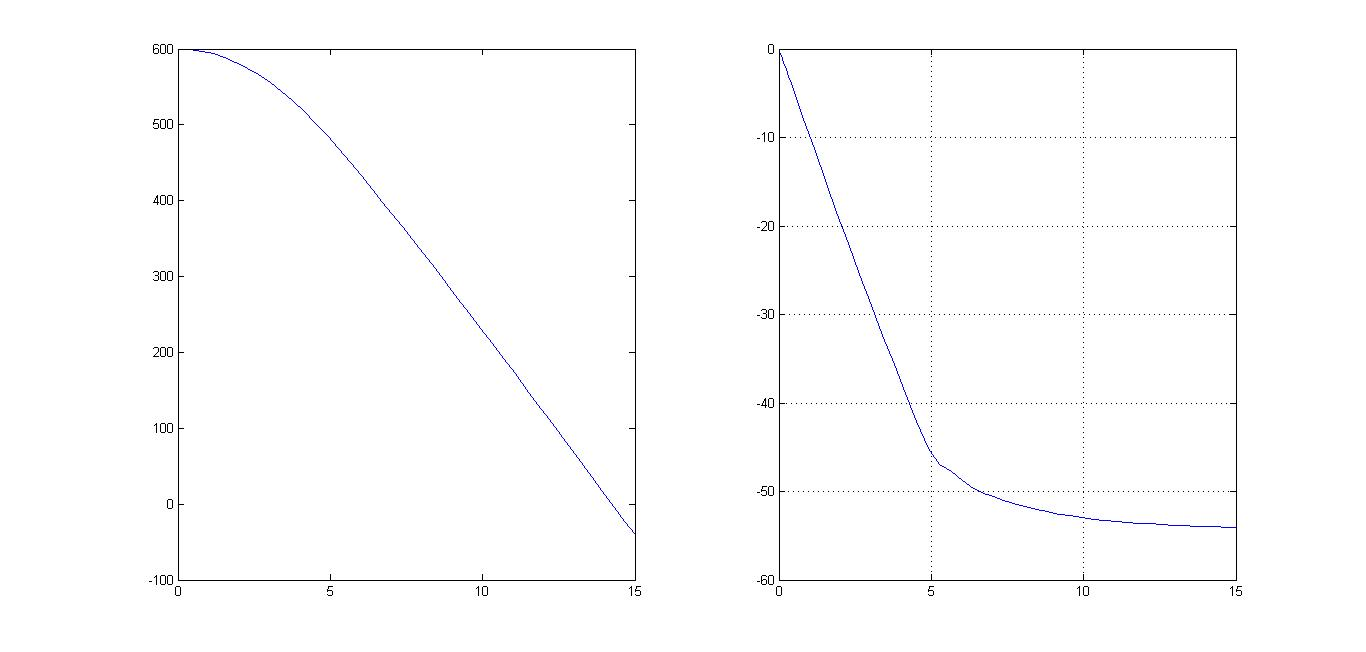
\includegraphics[width=0.8\textwidth]{./paracaidista.jpg}
\end{center}
\item Y de esta gr\'afica se puede responder que 
\begin{itemize}
\item El paracaida se abre a los 500 metros.
\item El paracaidista se demora 14 segundos en llegar al suelo.
\end{itemize}
\end{enumerate}
\end{enumerate}
\end{document}   
